\documentclass[t, notes, xcolor=table]{beamer}

\usepackage{wrapfig}
\usepackage{float}
% For tabs in verbatim
\usepackage{fancyvrb}

% Adjust position of the image
\usepackage[export]{adjustbox}

% set fonts
\usefonttheme{professionalfonts} % using non standard fonts for beamer
\usepackage{txfonts,mathptmx}

% set indend spacing for first and second level indentation
\setlength{\leftmargini}{0.5cm}
\setlength{\leftmarginii}{0.5cm}
\setlength{\leftmarginiii}{0.5cm}

% Set circles for bullets 
\setbeamertemplate{itemize items}[circle]

% colors
\usepackage{xcolor}

% multiple columns
\usepackage{multicol}

% todo lists
\usepackage{pifont}
\usepackage{amssymb}

% increase space between text and frame name
\addtobeamertemplate{frametitle}{}{\vspace{0.5em}}

%Information to be included in the title page:
\title{Using Blocking and Non-Blocking Statements}
\author{Nikola Petrovic}
\institute{University of Belgrade, School of Electrical Engineering}
\date{2022}



\begin{document}

\frame{\titlepage}

%%%%%%%%%%%%%%%%%%%%%%%%%%%%%%%%%%%%%%%%%%%%%%%%%%%%%%%%%%%%
\begin{frame}
\frametitle{Module Objective}

In this module we will use non-blocking assignments to model sequential design behaviour.
\newline

\textbf{Topics:}
\begin{itemize}
\item Blocking assignment introduction
\item Blocking assignments in sequential procedures
\item Non-blocking assignment introduction
\item Non-blocking assignments in sequential procedures
\item Assignments in combinational procedures
\item Mixing blocking and non-blocking assignments
\end{itemize}

\end{frame}
\note{
Out objective is to correctly choose between blocking and non-blocking assignments. To do that, we need to know more details about using blocking and non-blocking assignments in combinational and sequential procedures.

}

%%%%%%%%%%%%%%%%%%%%%%%%%%%%%%%%%%%%%%%%%%%%%%%%%%%%%%%%%%%%
\begin{frame}[fragile]
\frametitle{Blocking Assignment Introduction}

A blocking assignment blocks further execution until complete.
\begin{Verbatim}[commandchars=\\\{\}, tabsize=2]
\textcolor{purple}{		variable = [delay_control] expression}
\textcolor{purple}{		variable = [event_control] expression}
\end{Verbatim}
\begin{itemize}
\item By default completes immediately
\end{itemize}

\begin{figure}
    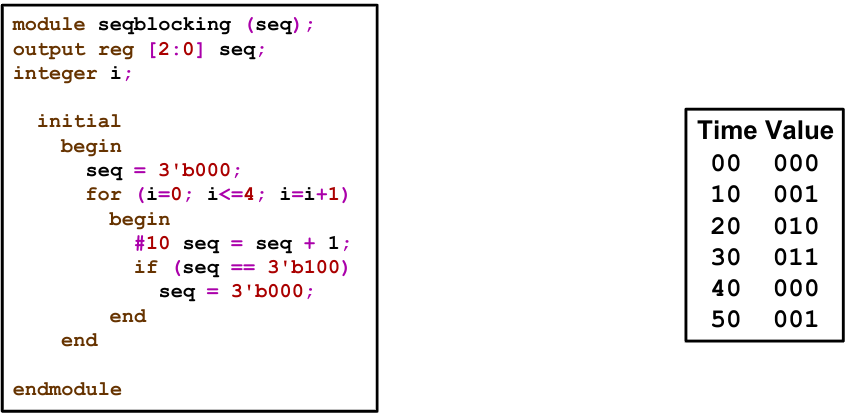
\includegraphics[width=0.95\textwidth]{img/07_block.png}
\end{figure}
\end{frame}
\note{
\scriptsize{
The simulator executes a blocking assignment by evaluating the right-side expression, retaining its value, and blocking further execution of the block until it updates the left-side variable. If the assignment includes an intra-assignment timing control, then the simulator updates the variable after timing control expires, and then continues block execution. If the assignment does not include intra-assignment timing control, then the simulator updated the variable immediately.
\newline

In this example, the \textit{for} loop increments the \textit{seq} signal every 10 time units. The update occurs before the next statement executes. The next statement tests the new value, and if the new value is 4, immediately resets it to 0. The value 4 has no duration, so does not appear in the sequence of monitored values.


}
}

%%%%%%%%%%%%%%%%%%%%%%%%%%%%%%%%%%%%%%%%%%%%%%%%%%%%%%%%%%%%
\begin{frame}
\frametitle{Blocking Assignments in Sequential Procedures}

\scriptsize{
\begin{multicols}{2}
Blocking assignments can lead to race conditions, specifically when the same event triggers multiple procedures.
\newline


\textbf{Examples:}
\begin{itemize}
\item Both procedures execute on the positive clock edge
\item Blocking assignments to a and b finish immediately upon statement execution.
\item But which statement executes first?
\item The value of b depends on which procedure executes first
\end{itemize}
\vfill
\columnbreak
\begin{figure}
    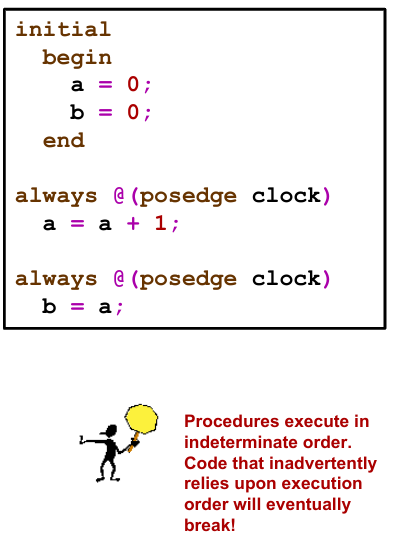
\includegraphics[width=0.45\textwidth]{img/07_block_seq.png}
\end{figure}
\end{multicols}
}
\end{frame}
\note{
\scriptsize{
Blocking assignments can lead to race conditions specifically when the same event triggers multiple procedures, that then execute in a non-deterministic order, such that a procedure can read a variable that another procedure may or may not have already written.
\newline

In this example, both procedural blocks unblock on the positive clock edge. The simulator can resume block execution in any order. The assignment statements use the blocking operator, so a race exists between the assignments to a an to b.
\begin{itemize}
\item If the simulator first executes the upper block, it updates \textit{a} to get the incremented value and then executes the lower block where it updates \textit{b} to get a new \textit{a} value.
\item If the simulator first executes the lower block, it updates \textit{b} to get the not yet changed \textit{a} value and then executes the upper block where it updates \textit{a} to get the incremented value.
\end{itemize}
The final \textit{b} value \textbf{does} depend on the procedure execution order.

}
}

%%%%%%%%%%%%%%%%%%%%%%%%%%%%%%%%%%%%%%%%%%%%%%%%%%%%%%%%%%%%
\begin{frame}
\frametitle{Blocking Assignment Order Affects Functionality}
\begin{figure}
    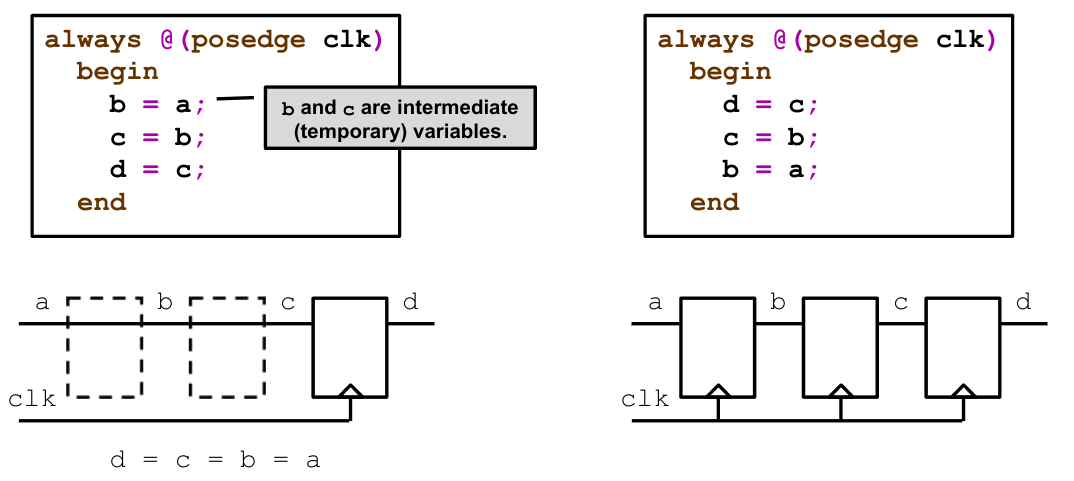
\includegraphics[width=0.95\textwidth]{img/07_block_order.png}
\end{figure}
\end{frame}
\note{
\tiny{
The left illustration uses blocking assignments:
\begin{itemize}
\item It assigns \textit{a} to \textit{b}, and immediately updates the \textit{b} value
\item  Then it assigns \textit{b} to \textit{c} and immediately updates the \textit{c} value
\item Finally, it assigns \textit{c} to \textit{d} and immediately updates the \textit{d} value
\end{itemize}

As each variable is written before it is read, all the variables have the value of \textit{a}. The \textit{b} and \textit{c} variables will not exist in a hardware implementation, as the \textit{d} variable provides the same value.
\newline

The right illustration also uses blocking statements, but it reorders the assignments:
\begin{itemize}
\item It assigns \textit{c} to \textit{d}, and immediately updates the \textit{d} value
\item  Then it assigns \textit{b} to \textit{c} and immediately updates the \textit{c} value
\item Finally, it assigns \textit{a} to \textit{b} and immediately updates the \textit{b} value
\end{itemize}

As the variables are read before they are written, all can have different values. All the variables will exist in hardware implementation.
\newline

This is an example of the position-dependent code. The statement order affects the functionality. We need to be aware of this issue, but it is not "bar" programming as such, because it is actually quite useful when deliberately done.
\newline

For this illustration, statement order would not affect functionality if the assignments were non-blocking.

}
}

%%%%%%%%%%%%%%%%%%%%%%%%%%%%%%%%%%%%%%%%%%%%%%%%%%%%%%%%%%%%
\begin{frame}[fragile]
\frametitle{Non-blocking Assignment Introduction}
A non blocking assignment schedules completion and does not block.
\begin{Verbatim}[commandchars=\\\{\}, tabsize=2]
\textcolor{purple}{		variable <= [delay_control] expression}
\textcolor{purple}{		variable <= [event_control] expression}
\end{Verbatim}
\begin{itemize}
\item By default completes when all executing blocks have blocked.
\end{itemize}
\begin{figure}
    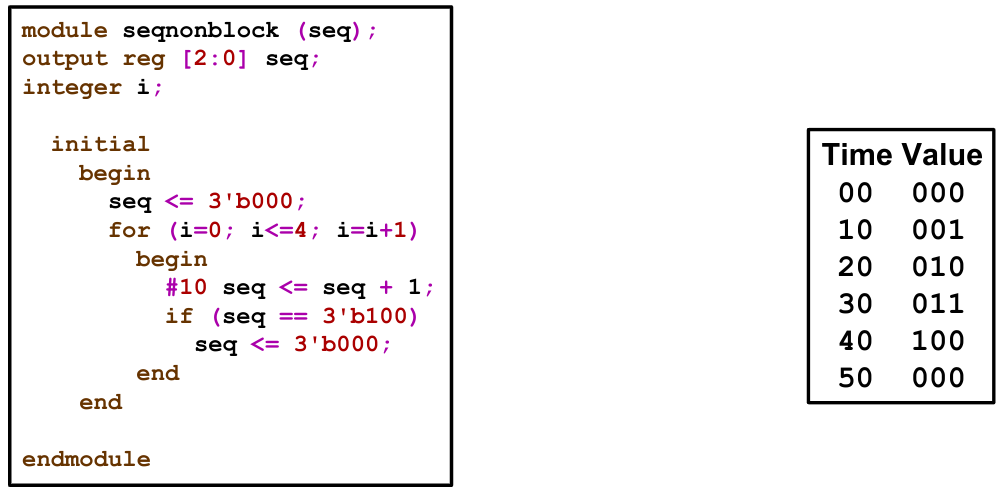
\includegraphics[width=0.95\textwidth]{img/07_nonblock.png}
\end{figure}
\end{frame}
\note{
\scriptsize{
The simulator executes a non-blocking assignment by evaluating right-side expression, retaining its value, scheduling the update, and continuing to execute the block until it encounters a blocking construct. The simulator schedules the variable update for a point in the simulation where all currently active blocks have executed up to the point where they are all blocked. This ensures that any other active block that reads the variable, reads the old value and not the new value.
\newline

In this example, the \textit{for} loop increments the \textit{seq} signal every 10 time units. The update does not immediately occur. The next statement tests the old value, and if the old value is 4, resets to 0. The value 4 has a duration of 10 time units, so does appear in the sequence of monitored values.

}
}

%%%%%%%%%%%%%%%%%%%%%%%%%%%%%%%%%%%%%%%%%%%%%%%%%%%%%%%%%%%%
\begin{frame}
\frametitle{Making Non-blocking Assignments in Sequential Procedures}
\scriptsize{
\begin{multicols}{2}

Non-blocking assignments \textit{avoid} race conditions, for example:
\begin{itemize}
\item Both procedures execute on the same positive edge clock
\item Assignments to "a" and "b" are scheduled
\item Assignment to "b" assigns the value of "a" from before the positive clock edge.
\end{itemize}
\vfill
\columnbreak
\begin{figure}
    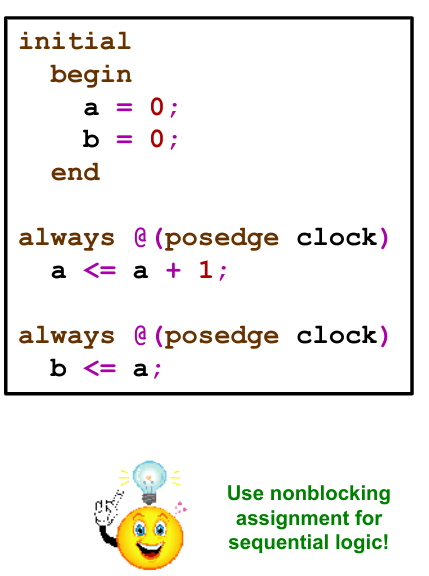
\includegraphics[width=0.45\textwidth]{img/07_nonblock_seq.png}
\end{figure}

\end{multicols}
}
\end{frame}
\note{
\scriptsize{
in this example, both procedural blocks unblock on the positive clock edge. The simulator can resume block execution in any order. The assignment statements use the non-blocking operator, so no race condition occurs.
\begin{itemize}
\item If the simulator first executes the upper block, it schedules an "a" variable update to get the incremented value and the "a" variable value does not yet change. The simulator then executes the lower block where it schedules a "b" variable update to get the old \textit{unchanged} "a" variable value.
\item If the simulator first executes the lower block, it schedules a "b" variable update to get the not yet changed "a" variable value. The simulator then executes the upper block, where it schedules an "a" variable update to get the incremented value.
\item After executing these and all other triggered blocks to the point where they all block, the simulator completes the non-blocking assignments to update the variable values.
\end{itemize}
The final "b" variable value does NOT depend upon execution order.

}
}

%%%%%%%%%%%%%%%%%%%%%%%%%%%%%%%%%%%%%%%%%%%%%%%%%%%%%%%%%%%%
\begin{frame}
\frametitle{Can Non-blocking Assignment Order Affect Functionality}
Non-blocking assignment order of appearance cannot affect functionality if:
\begin{itemize}
\item Statements are executed in the same simulation cycle
\item Each target is assigned only once
\item No target is assigned in any other procedural block
\item No blocking assignments are mixed with the non-blocking assignments
\end{itemize}
\begin{figure}
    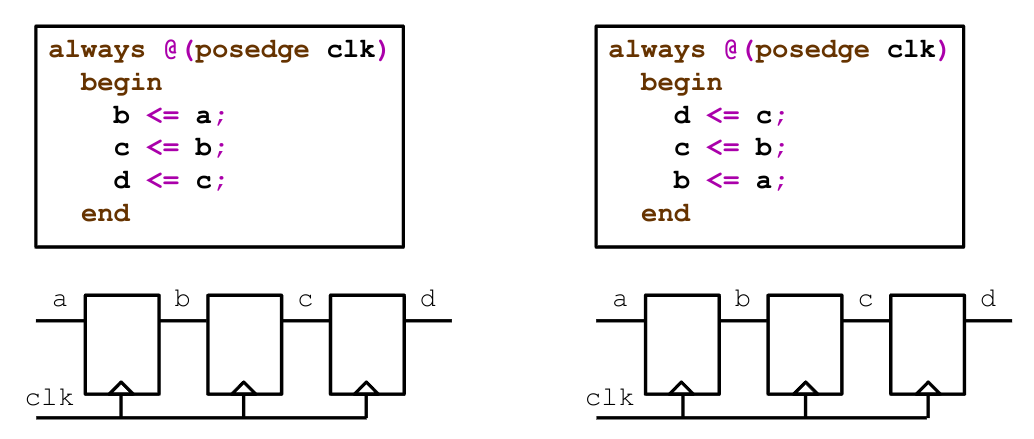
\includegraphics[width=0.95\textwidth]{img/07_nonblock_order.png}
\end{figure}
\end{frame}
\note{
here is the same illustration as previously , but utilizing non-blocking assignments. If we simply adhere to good programming practices, then the order of assignments appearance cannot affect functionality.

}

%%%%%%%%%%%%%%%%%%%%%%%%%%%%%%%%%%%%%%%%%%%%%%%%%%%%%%%%%%%%
\begin{frame}
\frametitle{Making Assignments to Temporary Variables}
\scriptsize{
\begin{multicols}{2}
We can use blocking assignments to intermediate (temporary) variables within sequential procedures.
\begin{itemize}
\item Declare temporary variables locally to discourage their use outside the block
\item Assign inputs to temporary variables with blocking assignment
\item Perform algorithm with temporary variables and blocking assignments
\item Assign temporary variables to outputs with non-blocking assignment
\end{itemize}
\vfill
\columnbreak
\begin{figure}
    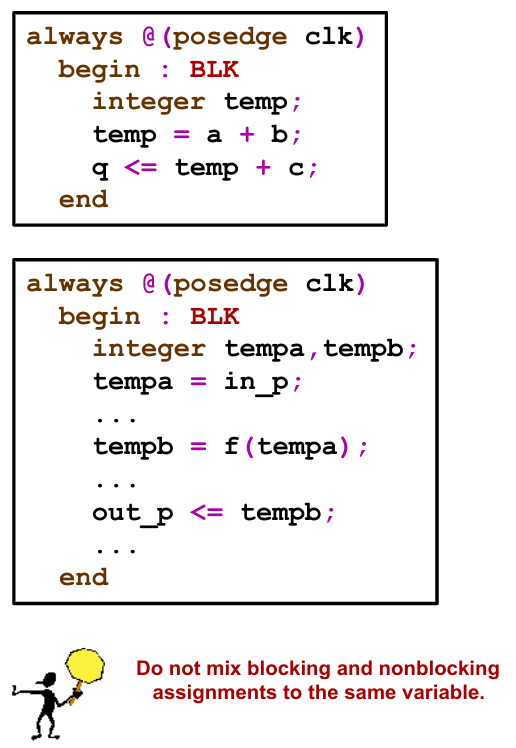
\includegraphics[width=0.45\textwidth]{img/07_block_temp.png}
\end{figure}
\end{multicols}
}
\end{frame}
\note{
\scriptsize{
We have previously seen that position dependent code is not "bad" programming as such, because it is actually quite  when deliberately done.
\newline

We can use blocking assignments to strictly temporary variables within sequential procedural blocks meant to represent sequential logic.
\newline

The usage model is to use blocking assignments, which complete immediately, to break a complex expression representing combinational logic into a series of simpler assignments to temporary variables. Out final assignment uses the non-blocking operator to assign the temporary result to the variable that represents the sequential hardware.
\newline

For the temporary variables to be truly temporary, they cannot be used anywhere other that that one block. This is impossible to enforce in the Verilog language, but we can make them less likely to be used elsewhere by declaring them locally. Recall that to declare local variables we need to name the block.

}
}

%%%%%%%%%%%%%%%%%%%%%%%%%%%%%%%%%%%%%%%%%%%%%%%%%%%%%%%%%%%%
\begin{frame}
\frametitle{Multiple Assignments and Assignment Type}
We can make multiple assignments to a variable within one procedure:
\begin{itemize}
\item All assignments to a variable should be the same type
\item Subsequent assignments override the previous assignment
\item Watch out for unintended results!
\end{itemize}

\begin{figure}
    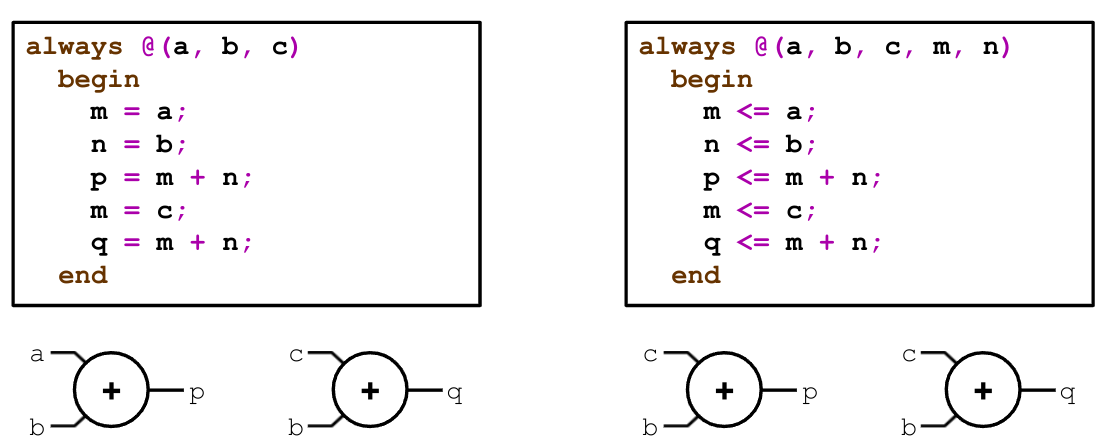
\includegraphics[width=0.95\textwidth]{img/07_multiple_assign.png}
\end{figure}
\end{frame}
\note{
\scriptsize{
We have previously seen that statement order affect functionality.
\newline

Assignment type can also affect functionality.
\newline

For blocking assignments, the simulator immediately updates the variable before continuing block execution. new values are immediately available until overwritten. In the blocking illustration, the simulator immediately updates the assignment of "a" to "m" and calculates a new value for "p" using the "a" value of "m". It then immediately updates the assignment of "c" to "m" and calculates a new value for "q" using the "c" value of "m".
\newline

For non-blocking assignments, the simulator schedules the variable update. New values are available only after update occurs. In the non-blocking illustration, the simulator schedules the assignment of "a" to "m" and immediately replaces it with a scheduled assignment of "c" to "m". Upon updating the "m" variable it gets the the value of "c" and not that of "a". The simulator re-executes the procedural block due to the transition of "m" and "n" and calculates new values for "p" and "q" that use the "c" value of "m".

}
}

%%%%%%%%%%%%%%%%%%%%%%%%%%%%%%%%%%%%%%%%%%%%%%%%%%%%%%%%%%%%
\begin{frame}
\frametitle{Module Summary}
\scriptsize{
Now we can use non-blocking assignments to model sequential design behaviour.
In this module, we described:
\begin{itemize}
\item Blocking and Non-blocking procedural assignment in sequential procedures
\begin{itemize}
	\scriptsize{
	\item In sequential procedures, the order of blocking procedural assignments affects the result.
	}
\end{itemize}
\item Blocking and Non-blocking assignment in combinational procedures
\begin{itemize}
	\scriptsize{
	\item In combinational procedures, blocking assignments are sufficient, but use them carefully.
	}
\end{itemize}
\item Mixing blocking and non-blocking assignment
\begin{itemize}
	\scriptsize{
	\item In a sequential procedure, make blocking assignments only to a temporary variables.
	}
\end{itemize}
\end{itemize}
}
\end{frame}
\note{
We can now correctly choose between blocking and non-blocking assignments. This module reviewed blocking and non-blocking assignments, and then examined how to use them in procedural blocks meant to represent combinational logic or sequential logic, and lastly explored issues with statement order and mixing blocking and non-blocking assignments in the same procedural block.

}
%%%%%%%%%%%%%%%%%%%%%%%%%%%%%%%%%%%%%%%%%%%%%%%%%%%%%%%%%%%%
\begin{frame}
\frametitle{Module Review}
\begin{enumerate}
\item What is the primary difference between blocking and non-blocking assignments?
\item Where should we use blocking assignments?
\item Where should we use non-blocking assignments?
\item Where can we legitimately mix blocking and non-blocking assignments?
\end{enumerate}
\end{frame}
\note{
\scriptsize{
\begin{enumerate}
\item What is the primary difference between blocking and non-blocking assignments?
\begin{itemize}
	\scriptsize{
	\item The blocking assignment operator blocks execution of subsequent statements until the assignment completes
	\item The non-blocking assignment operator calculates the RHS expression and schedules an update to the LHS variable.
	}
\end{itemize}
\item Where should we use blocking assignments?
\begin{itemize}
	\scriptsize{
	\item Use blocking assignments primarily in procedures that represent purely combinational logic
	}
\end{itemize}
\item Where should we use non-blocking assignments?
\begin{itemize}
	\scriptsize{
	\item Use non-blocking assignments for variables that represent storage, primarily in a procedure that represents sequential logic.
	}
\end{itemize}
\item Where can we legitimately mix blocking and non-blocking assignments?
\begin{itemize}
	\scriptsize{
	\item We can make blocking assignments to intermediate (temporary) variables in a sequential procedure.
	}
\end{itemize}
\end{enumerate}

}
}

%%%%%%%%%%%%%%%%%%%%%%%%%%%%%%%%%%%%%%%%%%%%%%%%%%%%%%%%%%%%
\begin{frame}
\frametitle{Module Exercise}
Code this circuit in two procedures in such manner that execution order does not affect the result.
\begin{figure}
    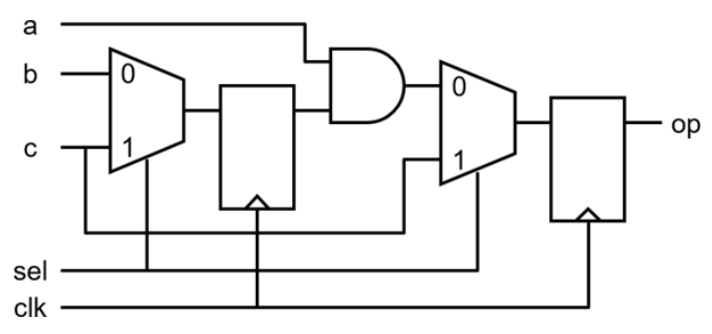
\includegraphics[width=0.95\textwidth]{img/07_exe.png}
\end{figure}
\end{frame}
\note{
\begin{figure}
    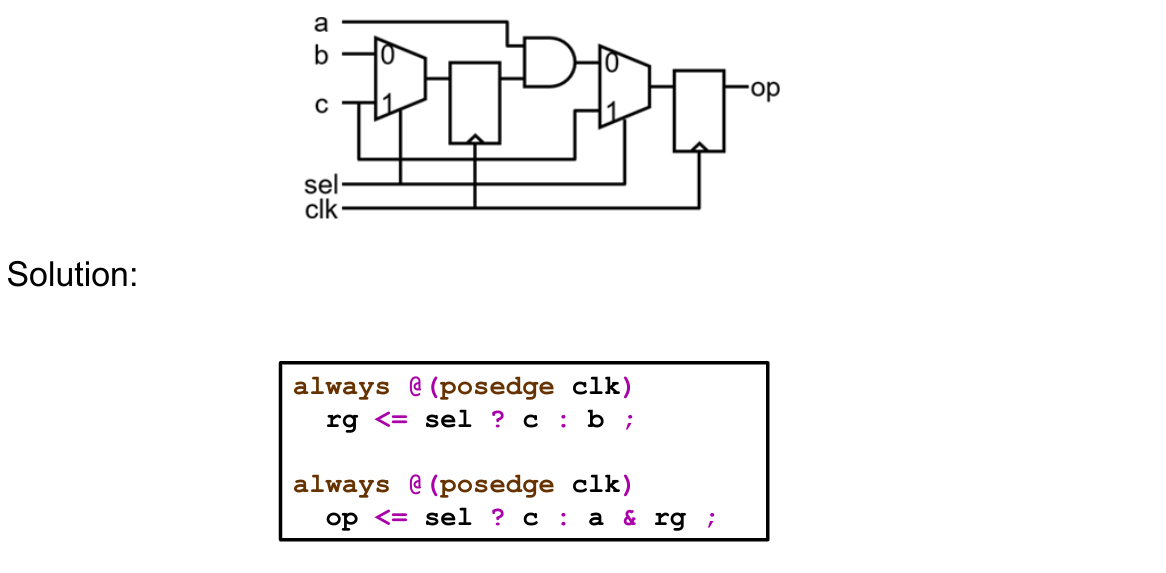
\includegraphics[width=0.95\textwidth]{img/07_exe_sol.png}
\end{figure}
}

%%%%%%%%%%%%%%%%%%%%%%%%%%%%%%%%%%%%%%%%%%%%%%%%%%%%%%%%%%%%
\begin{frame}
\frametitle{Lab}
Lab 8-1: Modeling a Generic Register
\begin{itemize}
\item Use non-blocking assignments while describing a register.
\begin{figure}
    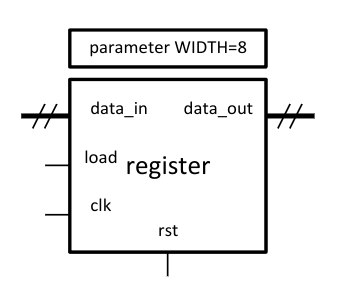
\includegraphics[width=0.35\textwidth]{img/07_lab.png}
\end{figure}
\end{itemize}
\end{frame}

%%%%%%%%%%%%%%%%%%%%%%%%%%%%%%%%%%%%%%%%%%%%%%%%%%%%%%%%%%%%
\begin{frame}
\frametitle{Test Your Understanding - 1}
The order in which we place blocking assignments within a procedure can affect functionality.
\begin{itemize}
\item[$\square$] True
\item[$\square$] False

\end{itemize}
\end{frame}
\note{

The order in which we place blocking assignments within a procedure can affect functionality.
\begin{itemize}
\item[$\boxtimes$] True
\item[$\square$] False

\end{itemize}
}

%%%%%%%%%%%%%%%%%%%%%%%%%%%%%%%%%%%%%%%%%%%%%%%%%%%%%%%%%%%%
\begin{frame}
\frametitle{Test Your Understanding - 2}
Non-blocking assignment statements are denoted by the symbol:
\begin{itemize}
\item[$\square$] \textless =
\item[$\square$] \textless\textgreater
\item[$\square$] \textgreater =
\item[$\square$] =
\end{itemize}
\end{frame}
\note{
Non-blocking assignment statements are denoted by the symbol:
\begin{itemize}
\item[$\boxtimes$] \textless =
\item[$\square$] \textless\textgreater
\item[$\square$] \textgreater =
\item[$\square$] =
\end{itemize}

}

%%%%%%%%%%%%%%%%%%%%%%%%%%%%%%%%%%%%%%%%%%%%%%%%%%%%%%%%%%%%
\begin{frame}
\frametitle{Test Your Understanding - 3}
The order in which we place non-blocking assignments within a procedure cannot affect functionality only if:
\begin{itemize}
\item[$\square$] Statements are executed in different simulation cycle
\item[$\square$] Target variable is assigned only once
\item[$\square$] Statements are executed in same simulation cycle
\item[$\square$] Blocking assignments are mixed with the non-blocking assignments
\item[$\square$] Target variable is not assigned in any other procedural block
\end{itemize}
\end{frame}
\note{
The order in which we place non-blocking assignments within a procedure cannot affect functionality only if:
\begin{itemize}
\item[$\square$] Statements are executed in different simulation cycle
\item[$\boxtimes$] Target variable is assigned only once
\item[$\boxtimes$] Statements are executed in same simulation cycle
\item[$\square$] Blocking assignments are mixed with the non-blocking assignments
\item[$\boxtimes$] Target variable is not assigned in any other procedural block
\end{itemize}

}



\end{document}
